\documentclass[a4paper,12pt]{article}
\usepackage{graphicx}
\usepackage{placeins}

\begin{document}

\title{WeatherApp | Documentation}
\author{Vilma Pirilä, Valma Haavisto, Aarni Akkala}

\maketitle

\section{Software Structure}

The WeatherApp consists of three main classes: WeatherApp (GUI), Events (event handlin) and API (API calls). 

\subsection{Class Diagram}

\begin{figure}[h]
    \centering
    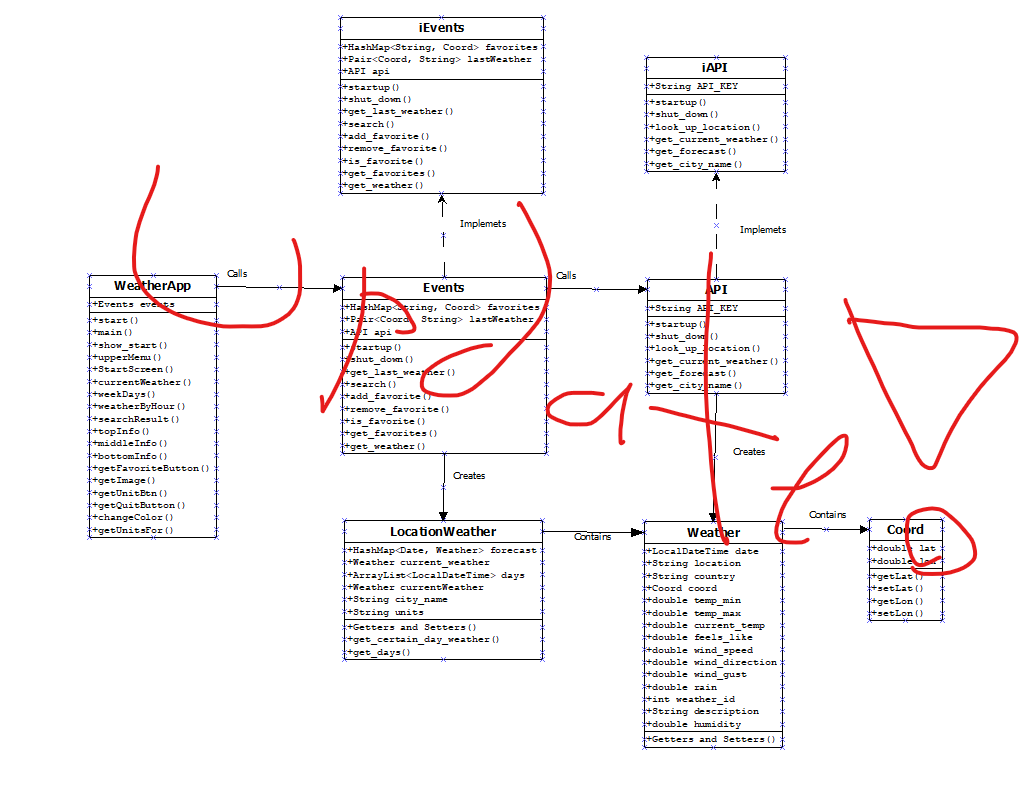
\includegraphics[width=1\textwidth]{class_diagram.png}
    \caption{UML Class Diagram of WeatherApp}
    \label{fig:class_diagram}
\end{figure}

\FloatBarrier

\subsection{Class Responsibilities}


\texttt{WeatherApp.java} is responsible for handling GUI element placement and event handling. It creates an \texttt{Events} object that manages storing favorites, the last searched location, and communicates with the API through an \texttt{API.java} object. The \texttt{Events.java} class implements the \texttt{iEvents.java} interface. 

The \texttt{API} class, implementing the \texttt{iAPI-java} interface, retrieves JSON files containing current weather data and forecasts for given locations from \texttt{openweathermap.org}. Additionally, it identifies coordinates and proper names for a given search term (up to 5 results).

These resulting JSONs are parsed to create \texttt{Weather} class instances, storing weather conditions (current or forecast) for a specific timestamp. \texttt{Events.java} then stores these \texttt{Weather.java} objects into \texttt{LocationWeather.java} class instances, representing all weather information for a particular location. For example, the current weather and a 4-day forecast for Tampere, Finland. The \texttt{Coord.java} class stores the latitude and longitude of a given location.

Refer to the Javadoc documentation for detailed information on the various functions within these classes.


\section{Project Functionality}

The WeatherApp encompasses a range of essential functionalities, each detailed in the "User Manual" section:

\begin{itemize}
	\item \textbf{Location Search:} Retrieve weather information from openweathermap.org by searching for a specific location.
	\item \textbf{Current Weather Display:} View real-time weather details for a selected location.
	\item \textbf{Forecast Information:} Access a comprehensive forecast, including hourly breakdowns for the current day and daily maximum and minimum temperatures for the next four days. Additionally, receive weather descriptions.
	\item \textbf{Favorites Management:} Easily add or remove locations to and from the favorites list for quick access.
	\item \textbf{Persistent Data:} Save the last accessed location and user favorites to a file, ensuring automatic retrieval and display when the application is relaunched.
	\item \textbf{Unit Customization:} Seamlessly switch between metric and imperial units to suit individual preferences.
\end{itemize}



\section{Implemented Classes}

List and briefly describe classes implemented by the team, specifying pre and post conditions where applicable.
List and briefly describe classes implemented by the team, specifying pre and post conditions where applicable.
List and briefly describe classes implemented by the team, specifying pre and post conditions where applicable.
List and briefly describe classes implemented by the team, specifying pre and post conditions where applicable.


\section{Division of Work}

Below are listed the responsibilities (agreed and actual) of each team member on this project:

\textbf{Vilma Pirilä:}
\begin{itemize}
    \item \texttt{WeatherApp.java:} Implemented the entire GUI class.
    \item \texttt{GUI weather icons:} Weather icons shown on GUI were made by Vilma.
\end{itemize}

\textbf{Valma Haavisto:}
\begin{itemize}
    \item \texttt{Events.java:} Implemented the entire class and test class for it.
    \item \texttt{LocationWeather.java:} Implemented part of the functions.
    \item \texttt{iEvents \& iAPI interfaces:} Planned interfaces of the three main classes.
    \item \texttt{Organizing team meetings:} Organized team meetings and created a communication platform on Telegram.
\end{itemize}

\textbf{Aarni Akkala:}
\begin{itemize}
    \item \texttt{API.java:} Implemented the entire class and test class for it.
    \item \texttt{iEvents \& iAPI interfaces:} Implemented interfaces of the three main classes.
    \item \texttt{Documentation.pdf:} Made documentation file and class diagram.
\end{itemize}


\section{User Manual}

This section provides a brief introduction to using the WeatherApp program.

\subsection{Running the app}

The main program is \texttt{WeatherApp.java}. Execute this file, and a graphical user interface should appear.

\begin{figure}[h]
    \centering
    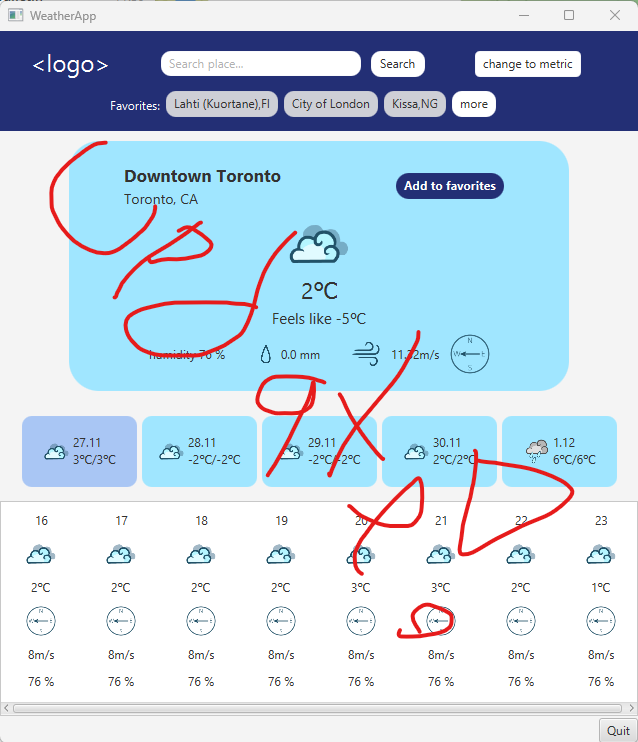
\includegraphics[width=0.9\textwidth]{weather_app_main_window.png}
    \caption{Main window launched when the program is run}
    \label{fig:main_window}
\end{figure}

\FloatBarrier

\subsection{Main window}

When on the main screen of WeatherApp, you can view the current weather conditions for the last accessed location. Under the current conditions, a forecast for the current day and the next four days is displayed. Clicking on these days reveals a detailed description of the weather conditions for each day (time, description icon, temperature, wind direction, wind speed, and rain probability).

\subsection{Searching for a location}

Utilize the topmost search bar to search for a location by entering its name (e.g., Tampere) and pressing Enter (or Search). A list of locations matching the search key is presented (up to five locations). By clicking on a result, the user is presented with the weather information and forecast for the chosen place on the main window, as previously described.

\subsection{Favorites}

The user can add a location to favorites by pressing "Add to favorites" or remove a location by pressing "Remove from favorites." Favorites are presented at the top in the "Favorites" section. From this list, the user can choose a location and receive its weather information. (Access more favorites by pressing "more.")

\subsection{Units}

There are two units available: metric or imperial. In metric, the temperature is in Celsius and wind speed in m/s. In imperial, the units are in Fahrenheit, and wind speed is in miles/hour.

\subsection{Closing program}

When the program is closed, the last viewed location and favorites are saved to memory and retrieved when the program is relaunched.


\section{Known Bugs and Missing Features}

Document any known bugs or features that are yet to be implemented.

\section{Conclusion}

Summarize the key points covered in the document.

\end{document}
